\chapter{Strutturazione dell'interfaccia grafica}
\minitoc\mtcskip

\section{Analisi del Client}\label{sec:clientanalisys}
\subsection{Interfaccia di avvio}

\begin{figure}[p]
 \centering
   \subfloat[][\emph{UIStart}.]{\label{fig:uistart}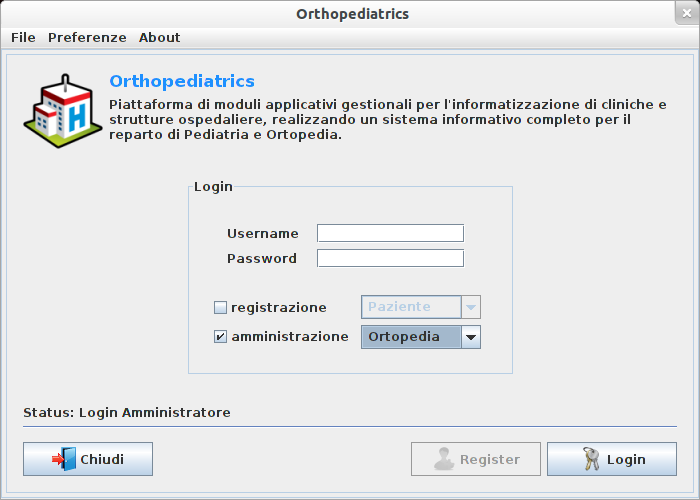
\includegraphics[scale=0.7]{GUI/UIStart}}\\
   \subfloat[][\emph{UIRegistration}.]{\label{fig:UIRegistration}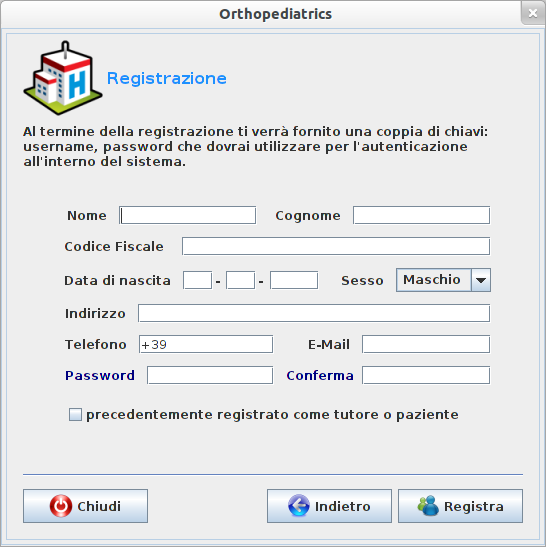
\includegraphics[scale=0.7]{GUI/UIRegistration}}\\
   \subfloat[][\emph{UIExitMessage}.]{\label{fig:UIExitMessage}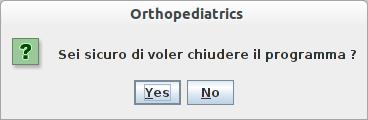
\includegraphics[scale=0.7]{GUI/UIExitMessage}}
   \caption{\emph{First UI Windows}.}
   \label{fig:clientimg_one}
\end{figure}

L'applicazione presenta un'interfaccia grafica semplice e intuitiva
da usare. All'avvio ciò che vede l'utente è rappresentato in Figura 
\vref{fig:clientimg_one}\subref{fig:uistart}.

L'utilizzo di Orthopediatrics è riservato a due tipi di utenti: Pazienti
e Amministratori. Per i pazienti, questi possono trovarsi in
due stati all'interno del sistema: registrati oppure non registrati.
Per effettuare la registrazione come paziente, è sufficiente selezionare
la casella {}``\emph{registrazione}'' ed automaticamente
viene abilitato il bottone {}``\emph{Register}'', premendo sul quale
il paziente viene rimandato ad una nuova visualizzazione in cui dovrà
effettuare l'inserimento dei dati personali, come mostrato in Figura 
\vref{fig:clientimg_one}\subref{fig:UIRegistration}.


Al termine di questa procedura, in caso di errore, il paziente verrà
informato di eventuali problemi; in caso di successo invece verrà
rimandato alla schermata precedente in modo da effettuare l'autenticazione
presso il sistema.

La fase di autenticazione avviene tramite \emph{Username} e \emph{Password}.
Se trattassi di pazienti questi devono inserire semplicemente le loro
credenziali e cliccare sul bottone {}``\emph{Login}'', dopo aver inserito
nel campo \emph{Username} il loro proprio codice fiscale.

Se l'utente che desidera accedere al sistema è un amministratore,
questo deve necessariamente selezionare la casella {}``\emph{amministratore}''
abilitando in questo modo il menù a tendina della scelta del reparto, selezionando
successivamente il reparto di appartenenza.

Un supporto agli utenti del sistema è fornito tramite \emph{lo stato}
({}``\textbf{Status}'') che informa l'utente, a seconda delle scelte
e opzioni effettuate, del tipo di operazione che si sta eseguendo.
In caso di problemi legati alla fase di login, lo status informa l'utente
di eventuali errori.

Dalla schermata iniziale l'utente può in qualunque momento decidere
di chiudere l'applicazione semplicemente cliccando sul bottone {}``\emph{Chiudi}'',
visualizzando la schermata di Figura \vref{fig:clientimg_one}\subref{fig:UIExitMessage}.



\subsection{Gestione delle prenotazioni}

\begin{figure}[!t]
 \centering
   \subfloat[][\emph{UIAdmin}.]{\label{fig:UIAdmin}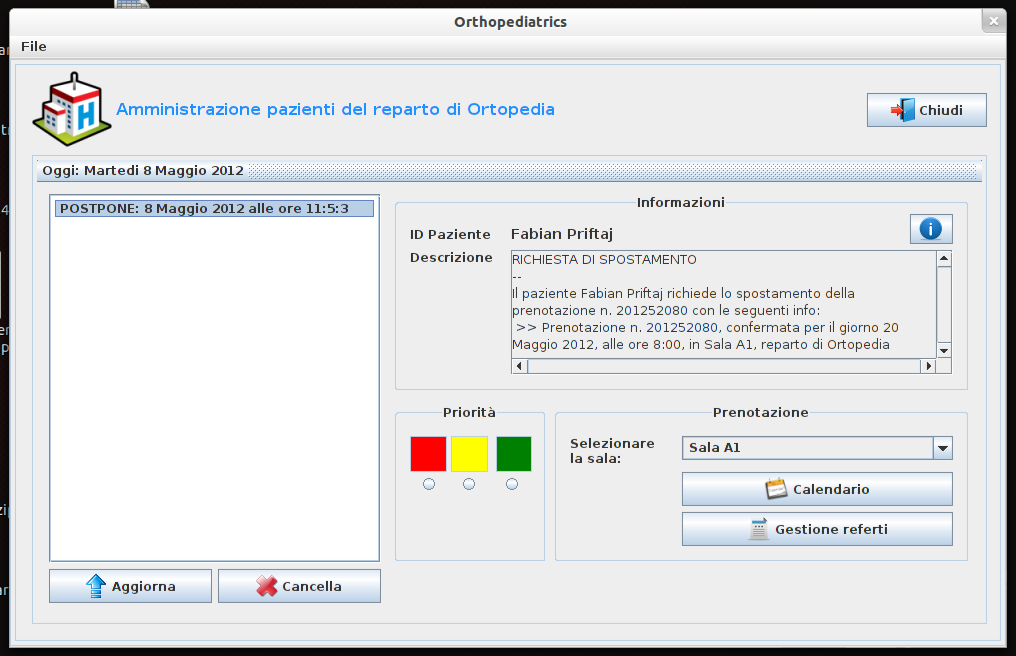
\includegraphics[scale=0.5]{GUI/UIAdmin}}\\
   \subfloat[][\emph{UICalendario (A Calendar View)}.]{\label{fig:UICalendario}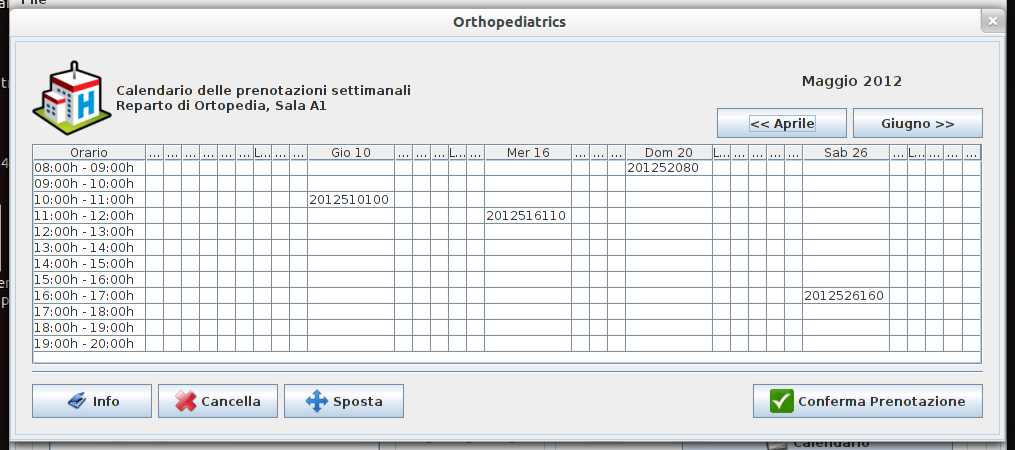
\includegraphics[scale=0.5]{GUI/UICalendario}}
 \caption{\emph{Administrator's UI Windows}.}
 \label{fig:uiadministrator_one}
\end{figure}

Se l'utente che effettua l'autenticazione presso il sistema è un amministratore,
allora l'interfaccia che il sistema mette a disposizione per la gestione
dei pazienti è rappresentata nella Figura \vref{fig:uiadministrator_one}\subref{fig:UIAdmin}.

Nella parte sinistra vengono visualizzate le richieste di prenotazione
dei pazienti. Selezionando una singola richiesta viene aggiornato
il campo {}``\emph{Informazioni}'' (nella parte destra) con alcune
semplici informazioni di base riguardanti il paziente. Cliccando sul
bottone \textbf{\emph{Altro}} si viene rimandati ad una nuova schermata
dove vengono visualizzate le informazioni complete del paziente.

L'amministratore in base alla descrizione della richiesta, stabilisce
una priorità espressa in tre diversi colori: rosso, giallo, verde.

In base alla priorità attribuita alla richiesta l'amministratore deve
stabilire il giorno in cui la visita deve avvenire. Cliccando sul
bottone \textbf{Calendario} si viene trasferiti ad una nuova schermata
rappresentata in Figura \vref{fig:uiadministrator_one}\subref{fig:UICalendario}.

Il calendario fornisce informazioni riguardanti un unica sala, che
deve essere scelta nella schermata precedente tra le sale disponibili
nel menu a tendina.

L'amministratore dopo aver selezionato la data opportuna, per confermare
la richiesta di prenotazione deve cliccare su \textbf{Conferma}, altrimenti
per tornare alla schermata precedente è sufficiente cliccare su \textbf{Indietro}.
In caso di informazioni mancanti, prima di procedere l'amministratore
verrà informato tramite messaggi di pop-up.


\subsection{Prenotazione della Visita}

\begin{figure}[p]
 \centering
   \subfloat[][\emph{UIPatient}.]{\label{fig:UIPatient}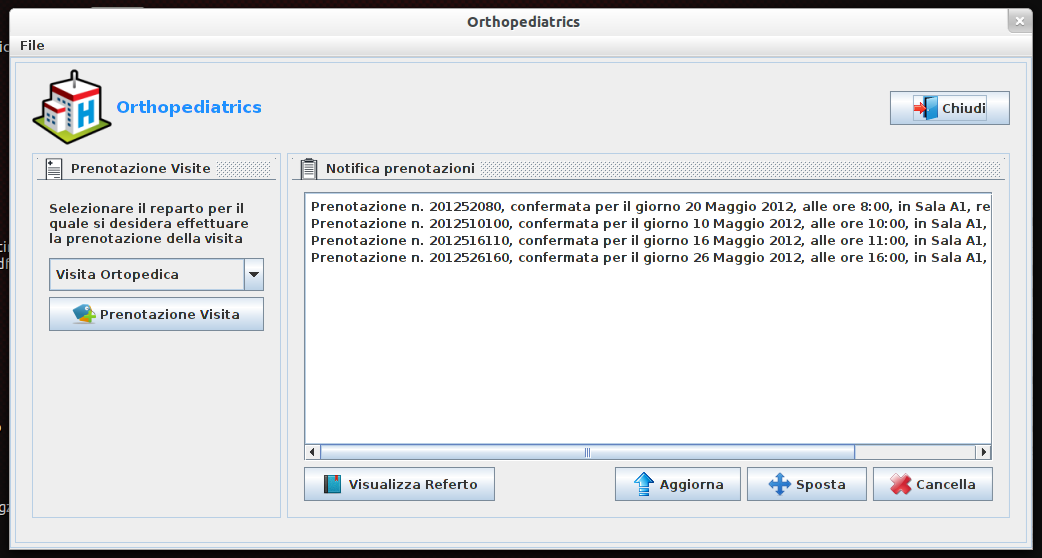
\includegraphics[scale=0.5]{GUI/UIPatient}}\\
   \subfloat[][\emph{UIPrenotazione (A Reservation View)}.]{\label{fig:UIPrenotazione}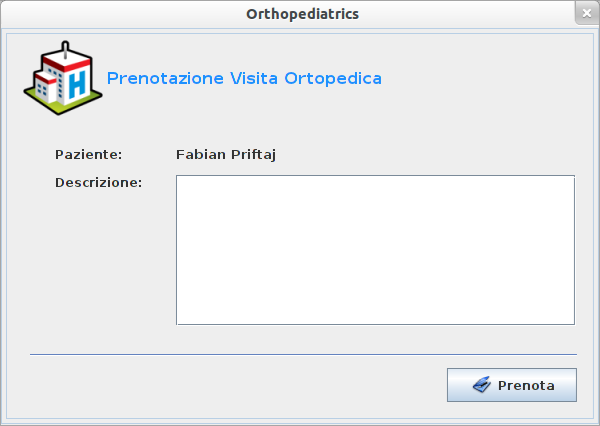
\includegraphics[scale=0.5]{GUI/UIPrenotazione}}\\
   \subfloat[][\emph{UITutorLogin}.]{\label{fig:UITutorLogin}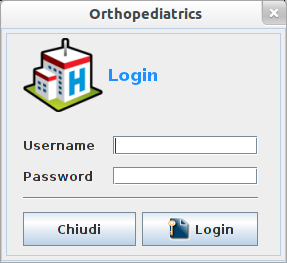
\includegraphics[scale=0.5]{GUI/UITutorLogin}}\\
 \caption{\emph{User's UI Window}.}
 \label{fig:uiuserwindow_one}
\end{figure}


La fase di prenotazione della visita è un attivita svolta dai pazienti
registrati presso il sistema. Il paziente può prenotare, cancellare
o spostare una visita utilizzando la seguente interfaccia messa a
disposizione dal sistema (Figura \vref{fig:uiuserwindow_one}\subref{fig:UIPatient}).

Inizialmente il paziente deve indicare il tipo di visita da effettuare:
\emph{ortopedica} o \emph{pediatrica}. In base a ciò viene selezionato
il reparto desiderato nell'area \emph{{}``Prenotazione Visite}''.
Per prenotare la visita, dopo aver scelto il reparto, è sufficiente
cliccare su \textbf{Prenota}. Successivamente viene mostrato una nuova
finestra in cui è visualizzato un campo di testo che il paziente dovrà
obbligatoriamente riempire con una descrizione dettagliata. Tale descrizione
deve essere sufficientemente chiara da permettere agli amministratori
di valutare le condizioni del paziente. 


Il sistema è utilizzato da paziente \emph{maggiorenni} e \emph{minorenni}.
In caso di pazienti con età inferiore a 18 è previsto un tutore. Questo
deve obbligatoriamente essere registrato all'interno del sistema.
Questo tutore è associato in fase di registrazione del paziente: Ogniqualvolta
un paziente minorenne tenta di prenotare una visita è richiesto
dal sistema un ulteriore autenticazione, che riguarda il tutore, tramite
la Figura \vref{fig:uiuserwindow_one}\subref{fig:UITutorLogin}.

Tutte queste possibili interazioni sono riassunte all'interno dei diagrammi
degli stati rappresentato in Figura \vref{fig:cliuistatechart_one}.

\begin{figure}[p]
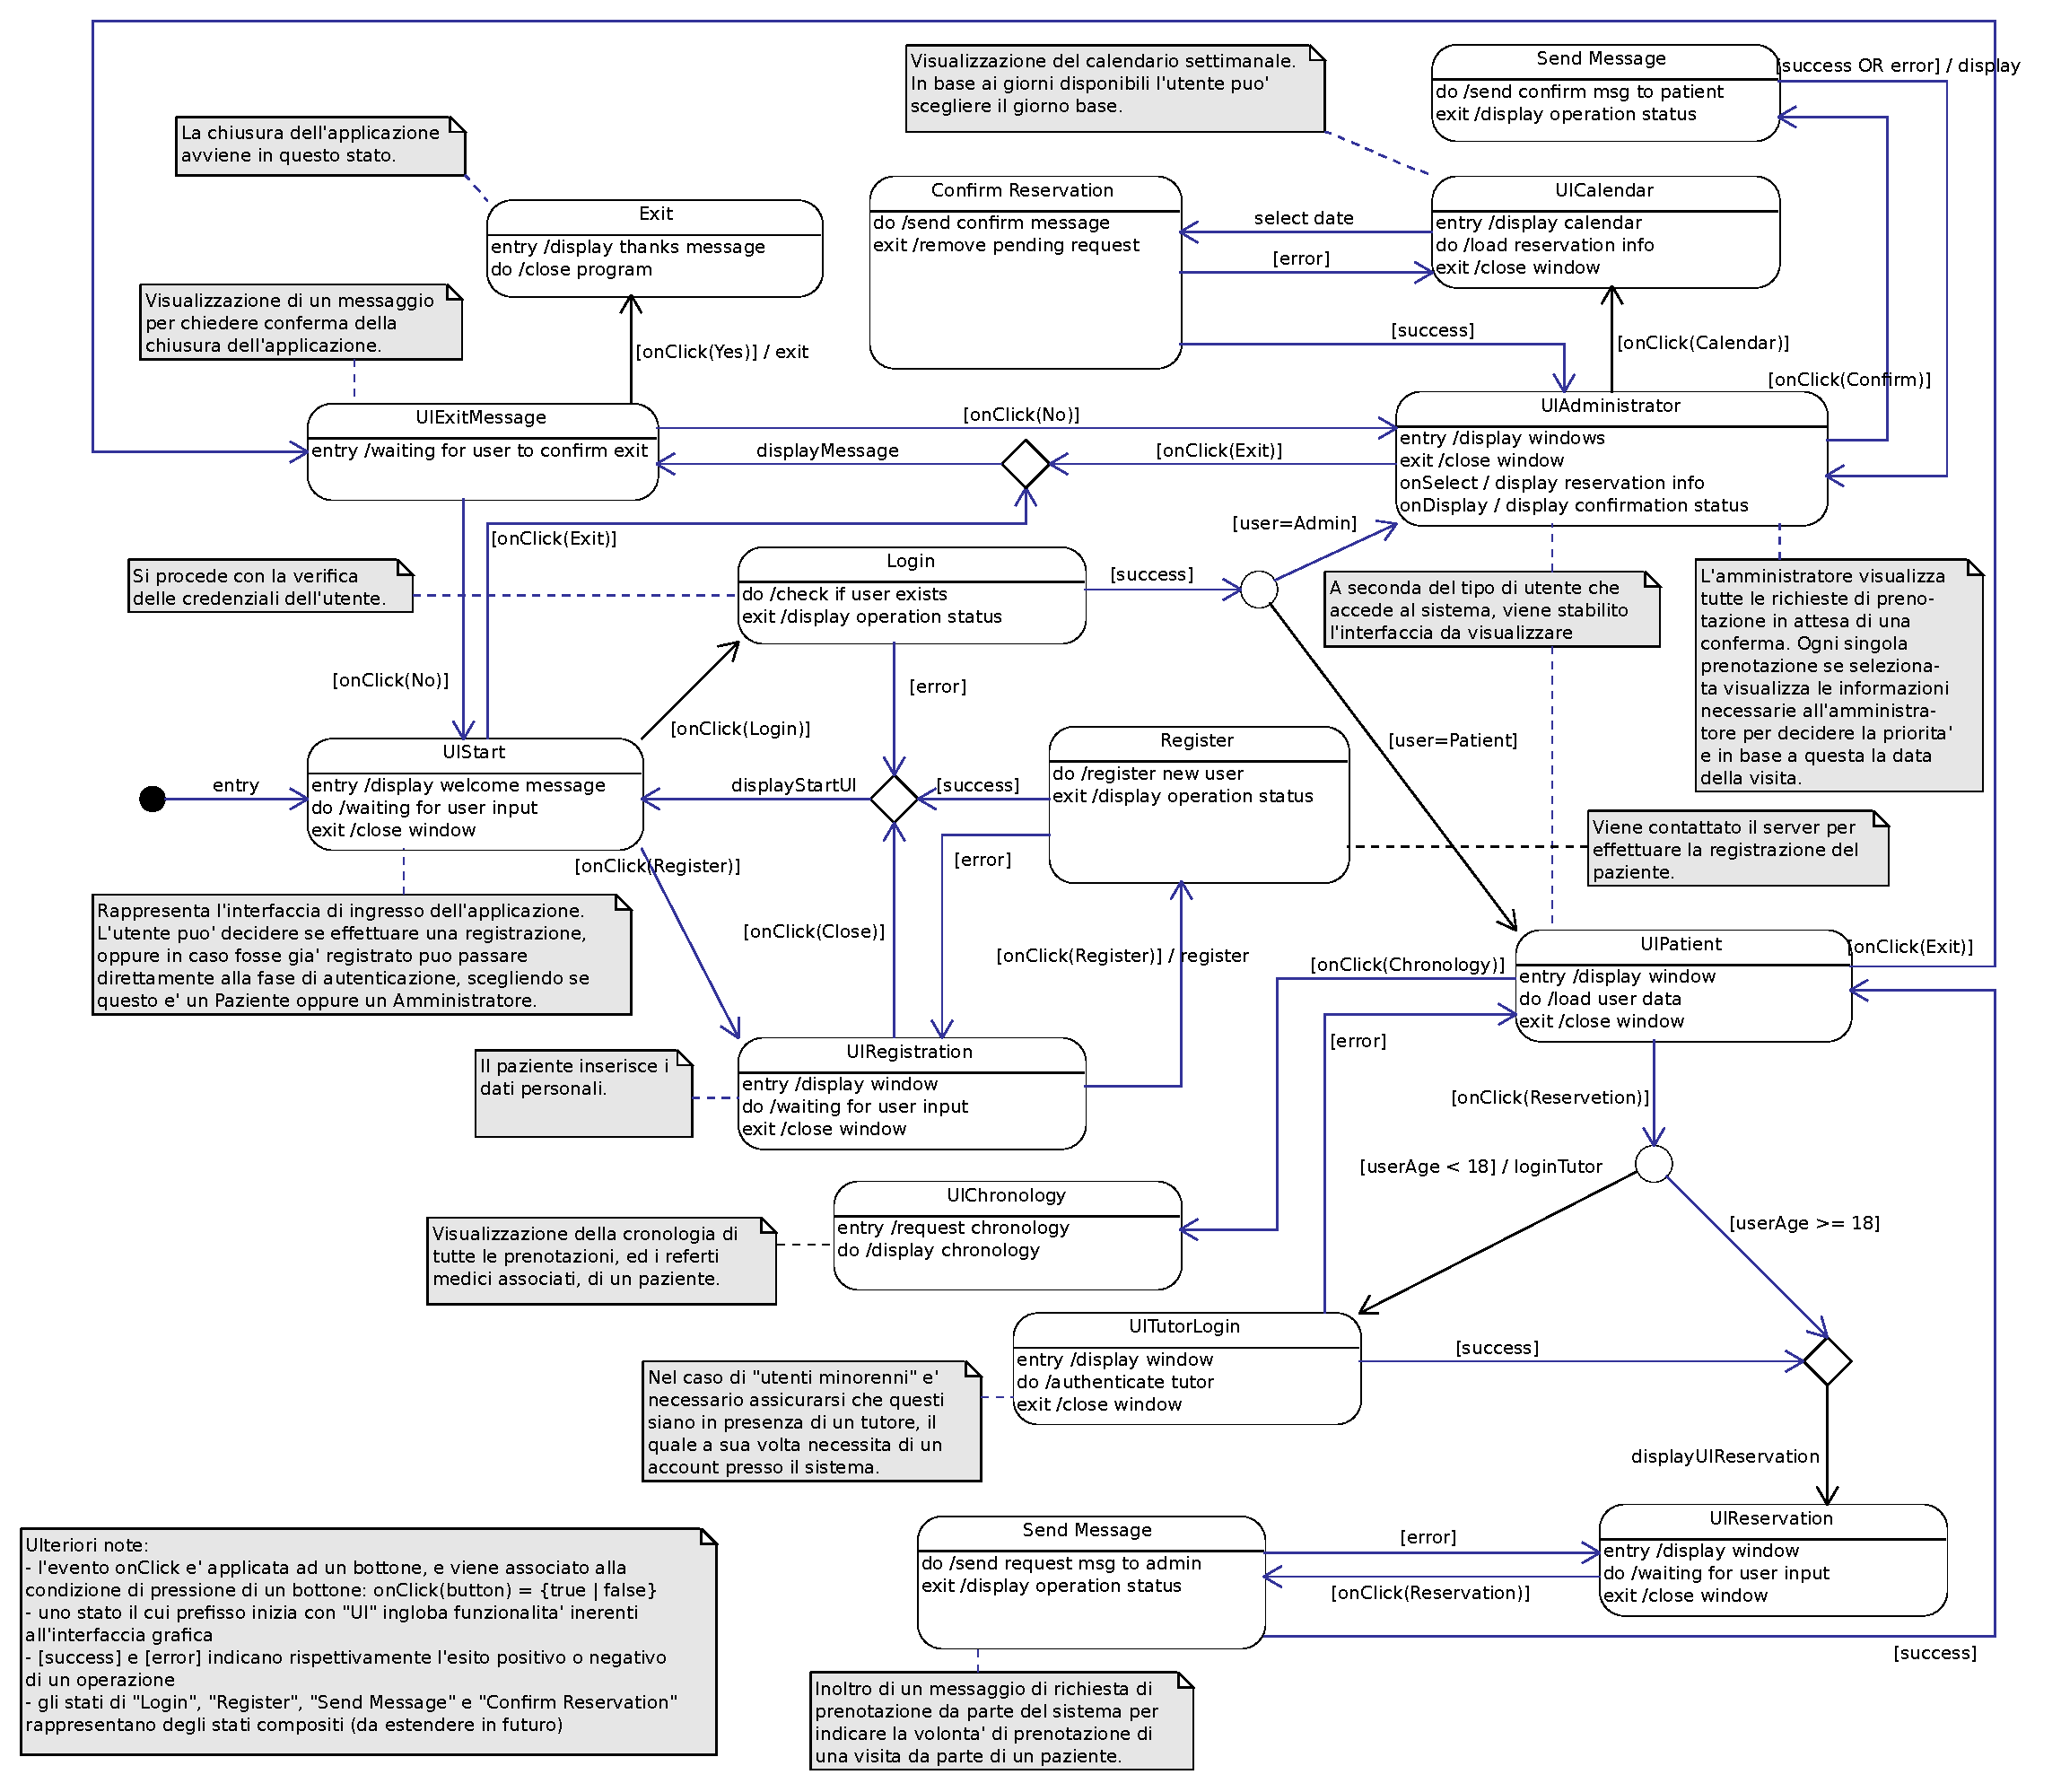
\includegraphics[scale=0.47,angle=90]{svgs/UIClient-Statechart-Diagrams}
\caption{\textit{Client UI Statechart. This statechat has the aim to link all the 
GUI screenshot that will follow}.}\label{fig:cliuistatechart_one}
\end{figure}
